\chapter{微分}
\label{ch:Differentiation}
进入到这章的学习的话,你已经开始进入数学的中等内容

\section*{学习目标}
\begin{todolist}
	\item 理解导数的作为曲线某一点的切线的斜率
	\item 掌握一阶导数和二阶导数的标记手段
	\item 掌握求算导数的一些法则,包括常数相乘,函数加减
	\item 利用\gls{chainrule}求算复合函数的导数
	\item 利用微分求算切线斜率,\gls{tangent}表达式,\gls{normal}表达式
	\item 利用微分求算函数的递增递减性质
	\item 利用微分求算相关变化率
	\item 利用微分求算\gls{stationary},并确定性质
\end{todolist}
\clearpage

\section{导数的来源和求算}
\label{sec:Derivative}
对于任意的函数图像,在某点处做切线,切线的斜率就是\gls{derivative}。
其标记手段为:
\[
	\frac{\mathrm{d} y}{\mathrm{d} x} \quad f'(x) \quad \frac{\mathrm{d} f}{\mathrm{d} x}
\]

\subsection*{$x^n$的导数}
\label{subsec:Derivative for Power}
对于幂次函数$x^n$。其导数为:
\[
	\frac{\mathrm{d}}{\mathrm{d} x}x^n = nx^{n-1}
\]

\subsection*{导数的求算法则}
\label{subsec:Operation Rules with derivative}
考试当中的函数必定不是这么简单的。需要了解一下的方法
\subsubsection*{加减以及数乘法则}
一般会通过多个函数进行一些运算。因此有如下的求导法则:
\begin{align*}
	\frac{\mathrm{d} (f\pm g) }{\mathrm{d} x} &=\frac{\mathrm{d} f}{\mathrm{d} x} \pm \frac{\mathrm{d} g}{\mathrm{d} x}\\
	\frac{\mathrm{d} C\cdot f}{\mathrm{d} x} &=C \cdot \frac{\mathrm{d} f}{\mathrm{d} x}
\end{align*}

\begin{ExampleBox}
Find the derivative of $y=3x^5-4x^2+8x+9$
\tcblower
将该函数分解为四个部分$3x^5$,$-4x^2$,$8x$,$9$。该函数的导数可以认为是这四部分的导数之和(差)
\begin{align*}
\frac{\mathrm{d} x^5}{\mathrm{d} x} &= 5\cdot x^4\\
\frac{\mathrm{d} 3x^5}{\mathrm{d} x}&= 3\times 5\cdot x^4
\end{align*}
同理可得到其他部分的导数为$-8x$,$8$,$0$。因此
\[
	\frac{\mathrm{d} y}{\mathrm{d} x}=15x^4-8x+8
\]
\end{ExampleBox}

\subsubsection*{链式法则}
\gls{chainrule}是最为重要的求导法则,用来求算复合函数的导数,利用了differential的传递性。其形式如下:
\[
	\frac{\mathrm{d} y}{\mathrm{d} x} =\frac{\mathrm{d} y}{\mathrm{d} u}\times \frac{\mathrm{d} u}{\mathrm{d} x}  
\]
但是运用该法则较难的地方是明确中间变量$u$。能够识别目标函数是有哪两层函数混合而来的。
可以查看此\href{https://www.bilibili.com/video/BV1qW411N7FU}{3B1B}的微积分视频当中的\href{https://www.bilibili.com/video/BV1qW411N7FU?p=4}{直观理解链式法则}。辅助自己记忆。

\begin{ExampleBox}
Find the derivative of $y=(x+x^3)^3$
\tcblower
Let $u=(x+x^3)$, then $y=u^3$.\\
First $\frac{\mathrm{d} y}{\mathrm{d} u} = 3\cdot u^2$\\
Second $\frac{\mathrm{d} u}{\mathrm{d} x} = 1+3x^2$\\
Finally 
\begin{align*}
\frac{\mathrm{d} y}{\mathrm{d} x} &=\frac{\mathrm{d} y}{\mathrm{d} u}\times \frac{\mathrm{d} u}{\mathrm{d} x}\\
		&=3u^2\times (1+3x^2)\\
		&=3(x+x^3)^2(1+3x^2)
\end{align*} 
\end{ExampleBox}

\begin{TaskBox}
尝试将$y=(x+x^3)^3$利用二项式展开,再进行求导。将求导后的结果与$3(x+x^3)^2(1+3x^2)$展开的结果进行比对,检验这两种方案求算的导数是否一致
\end{TaskBox}
\clearpage

\section{切线和法线}
\label{sec:Tangent Line}
由于之前已经说过,导数就代表切线的斜率,因此求导之后,就可以表示这些切线的表达式了。

\subsection*{切线}
对于某一个函数$y=f(x)$,其函数图像上存在一点为$(a,f(a))$。因此通过这个点绘制的切线,可以使用\gls{dxs}进行表示。可以写作$y-f(a)=m(x-a)$。因此还差该切线的斜率$m$就好。而根据导数的定义,$m=f'(a)$
因此,切线的表达式最后必定可以写成如下形式:
\[
	y-f(a)=f'(a) (x-a) \quad \text{or}\quad y-y_0=\frac{\mathrm{d} y}{\mathrm{d} x}\bigg |_{x_0} \cdot  (x-x_0)
\]
因此这种类型的题目只需要确定,切点的\emph{横纵}坐标$(a,f(a))$,或者$(x_0,y_0)$,以及\emph{导数},带入到点斜式当中即可。

\begin{ExampleBox}
Find the tangent of curve $y=2(3x-1)^{-\frac{1}{3}}$ at $x=\frac{2}{3}$.\\
\mbox{}\hfill Adapted from $2018$ winter paper$13$
\tcblower
首先确定切点的坐标 为$\left(\frac{2}{3},2\right)$\\
然后确定导数表达式
\[
	\frac{\mathrm{d} y}{\mathrm{d} x}=2\times -\frac{1}{3}(3x-1)^{-\frac{1}{3}-1}\times 3
\]
将切点的横坐标$-\frac{1}{3}$带入即可得到导数值为$-2$。\\
最后用点斜式进行切线的表示即可
\[
	y-2=-2 \times \left(x-\frac{1}{3}\right)
\]

如下图
\begin{figure}[H]
\centering
\includegraphics[width=0.8\textwidth]{tangentline}
\caption{原函数与切线图像}
\end{figure}
\end{ExampleBox}


\subsection*{法线}
\gls{normal}也是一个常考的考点,法线和切线都通过切点,并且互相\emph{垂直}。因此两条线的斜率互为负倒数。因此同样利用点斜式的方式,经过$(a, f(a))$的法线
\[
	y-f(a)=-\frac{1}{f'(a)}\cdot (x-a)
\]

如下图所示:
\begin{figure}[H]
\centering
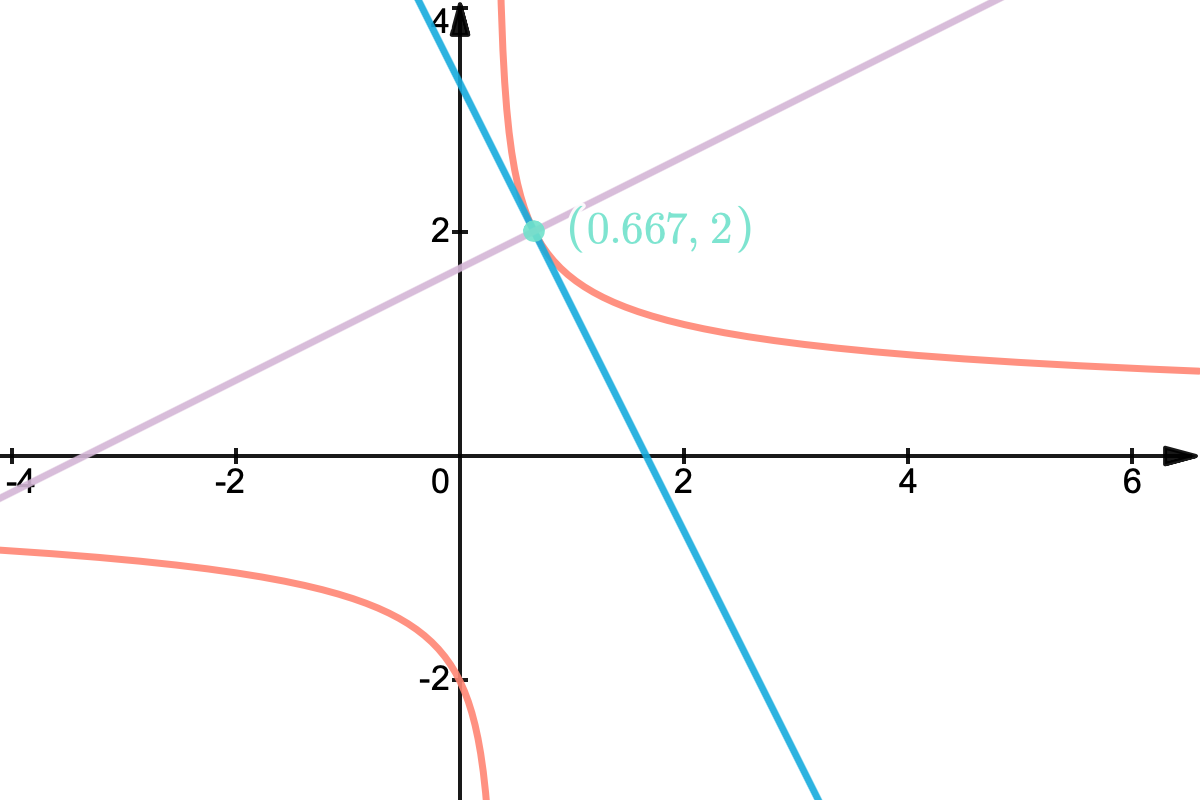
\includegraphics[width=0.8\textwidth]{normalline}
\caption{函数图像中的经过同一个点的切线与法线}
\end{figure}

\begin{TaskBox}
求算上图中紫色的法线的表达式。
\end{TaskBox}
\clearpage


\section{导数的应用}
\label{sec:Application of derivative}
微分求导是一门及其实用的学科,是数学分析的究极杀器之一。

\subsection*{函数的增减性}
不难发现,当一个函数的递增的时候,绘制的切线都是倾斜朝上的;而当函数递减的时候,绘制的切线都是倾斜朝下的。因此导数的正负性和函数的\gls{mono}是息息相关的。

\begin{SummBox}
如果$\frac{\mathrm{d} y}{\mathrm{d} x} > 0$,原函数递增\\
如果$\frac{\mathrm{d} y}{\mathrm{d} x} < 0$,原函数递减
\end{SummBox}

\subsection*{函数图像驻点}
在上一小节中,我们没有讨论当导数为$0$,也就是切线为水平直线的时候的情况,因为这些地方被称之为\gls{stationary}。是研究一个函数图像较为重要的控制点。

\begin{definition}
Stationary Point is anywhere in the curve where the derivative of it, $\frac{\mathrm{d} y}{\mathrm{d} x}$, is \emph{zero}。 
\end{definition}

\subsection*{二阶导数}
由于一般求导之后的结果$\frac{\mathrm{d} y}{\mathrm{d} x}$也是一个关于$x$的函数,因此该函数可以继续求导,再求导一次之后的结果称之为二阶导数。计作
\[
	\frac{\mathrm{d}^2 y}{\mathrm{d} x^2} \qquad f''(x)
\]

\begin{ExampleBox}
Find the second order derivative of $y=3x^5-4x^2+8x+9$.
\tcblower
首先求算一阶导数 $\frac{\mathrm{d} y}{\mathrm{d} x}$为:
\[
	\frac{\mathrm{d} y}{\mathrm{d} x}=15x^4-8x^2+8+0
\]
再求算二阶导数为:
\[
	\frac{\mathrm{d}^2 y}{\mathrm{d} x^2}=4\times 15x^3-2\times 8x+0
\]
\end{ExampleBox}


\subsection*{驻点的极值}
分辨一下这两个不同类型的驻点。
\begin{figure}[H]
\centering
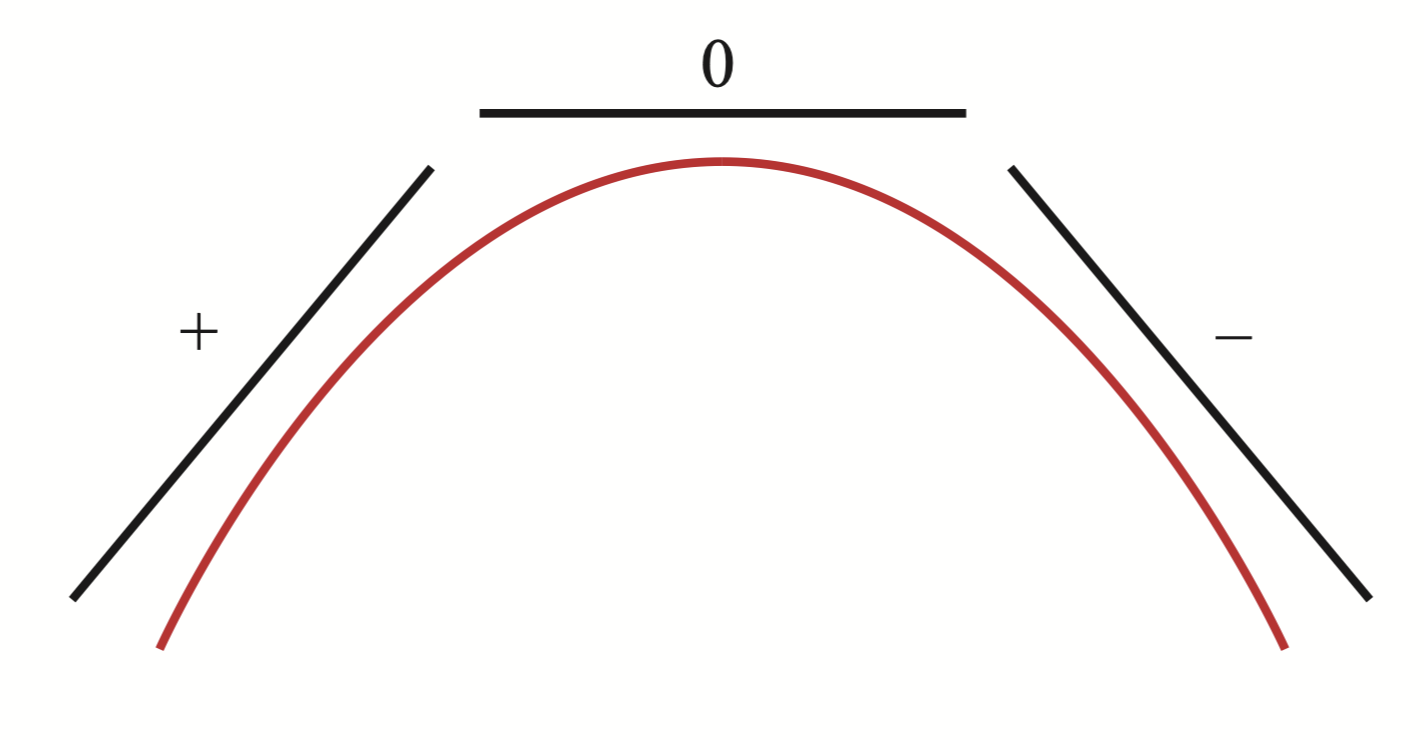
\includegraphics[width=0.45\textwidth]{maximum}
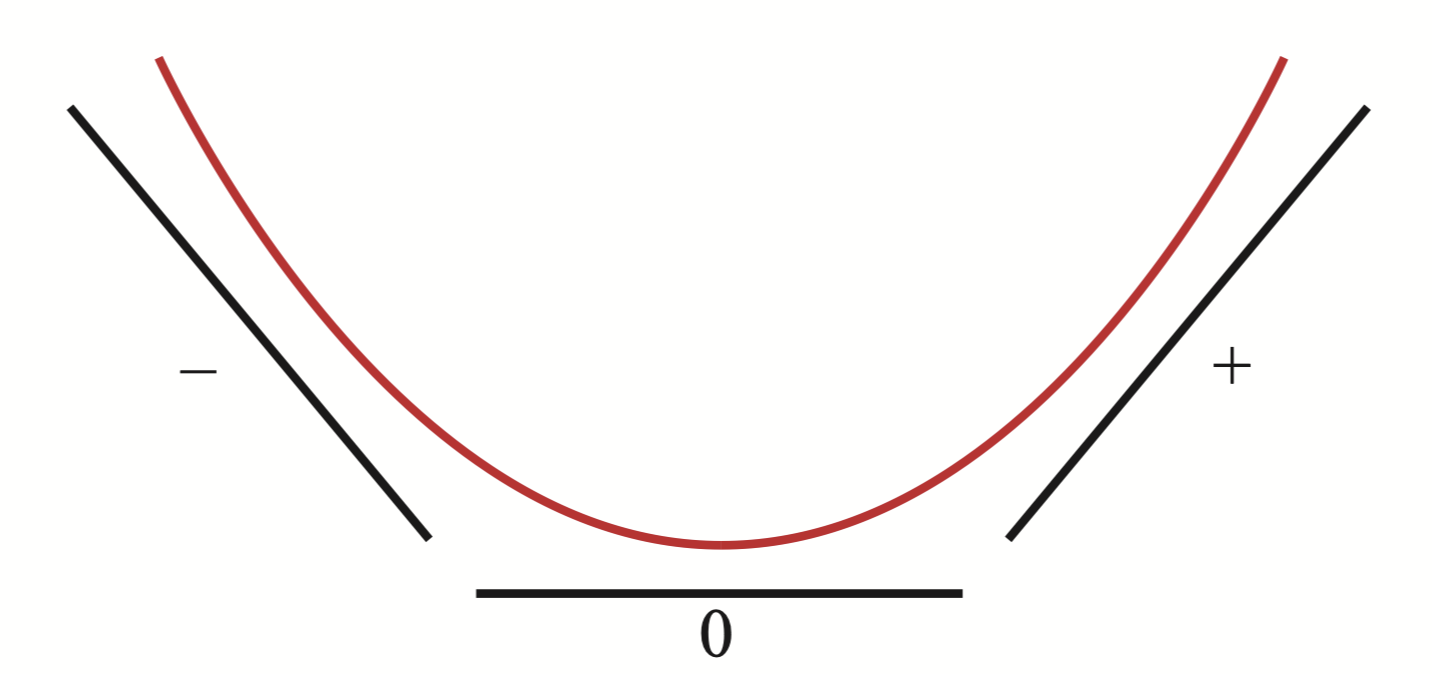
\includegraphics[width=0.45\textwidth]{minimum}
\caption{极大值和极小值点}
\end{figure}

函数在这两个点上都是一阶导数为$0$的,但是一个为极大值,另一个是极小值。原因是在极大值左侧,一阶导数都是正的,在极大值的右侧,一阶导数都是负值。也就是说一阶导数在递减,回顾一下,如果一阶导数\emph{递减}的话,其实就是等价于二阶导数为\emph{负值}。

同理可以推测,当驻点为极小值时,二阶导数为\emph{正值}。


因此确定一个函数的极大值极小值的过程如下
\begin{SummBox}
1.求算\fbox{$\frac{\mathrm{d} y}{\mathrm{d} x}=0$}的结果,\\
2.将$x$的值带入到其二阶导数$\frac{\mathrm{d}^2 y}{\mathrm{d} x^2}$中,\\
3.如果二阶导为\emph{正值};则函数在该点则为极小值点。如果二阶导数为\emph{负值},则函数在该点处为极大值点,\\
4.将$x$值带入到函数表达式中,即可得到$y$值。并说明是极大值还是极小值。
\end{SummBox}

\subsection*{相关变化率}
\label{subsec:Connected Rate of Change}

必定会有两个量随时间发生变化假设为$A$和$B$。在解决这一类问题时必定会利用到chain rule,因此可以直接写出

\[\frac{\mathrm{d} A}{\mathrm{d} t}=\frac{\mathrm{d} A}{\mathrm{d} B}\cdot \frac{\mathrm{d} B}{\mathrm{d} t}\]去题目当中找寻给定的rate of change,以及$A$和$B$之间的函数关系就可以了。

\begin{ExampleBox}
A curve is such that $\frac{\mathrm{d} y}{\mathrm{d} x}=2-8(3x+4)^{-\frac{1}{2}}$. A point $P$ moves along the curve in such a way that the $x$-coordinate is increasing at a constant rate of $0.3$ units per second. Find the rate of change of the $y$-coordinate in terms of $x$. \\
\makebox{}\hfill adapted from 2016 spring paper11
\tcblower
首先,明确一下题目中求算的是$y$坐标的变化率,计作$\frac{\mathrm{d} y}{\mathrm{d} t}$,给定的条件是$x$坐标的变化率$\frac{\mathrm{d} x}{\mathrm{d} t}=3$。因此利用导数求算的链式法则:
\[
	\frac{\mathrm{d} y}{\mathrm{d} t} = \frac{\mathrm{d} y}{\mathrm{d} x} \cdot \frac{\mathrm{d} x}{\mathrm{d} t}
\]
即可。
因此最后答案为$\frac{\mathrm{d} y}{\mathrm{d} t}=0.6-2.4(3x+4)^{-\frac{1}{2}}$
\end{ExampleBox}





